\documentclass{article}
\usepackage{fancyhdr,geometry,subfig,hyperref,graphicx,psfrag,amsfonts,wrapfig,mathtools}
\title{Mandatory exercise 2 \\ Signal and Image Processing 2012}
\author{Jens P. Raaby \\
\url{frn617@diku.dk}}

\begin{document}
\maketitle

\section*{Question 2.1 - Filtering Function}
I have implemented a simple Fourier-domain filtering package as a MATLAB function, applyFilter. This takes as parameters the image (in the form of a matrix), a filter (either spatial, in which case it will be Fourier transformed, or Fourier)  as well as a boolean option to visualise.

The steps taken by the applyFilter function are as follows:
The input image is converted to a matrix of double precision numbers. It's size is calculated and from that the padding size is also found (giving a padded size which is 4 times larger than the original). Then a padded version of the image is created (all outside areas are set to have a value of 0), and this is Fourier transformed.

Subsequently the filter is checked - if it is in the spatial domain the Fourier transform is calculated and shifted such that the filter is symmetric and padded to the same size as the padded image. 

Filtering is performed by multiplying each pixel with the corresponding filter value, both of which are in the Fourier domain. To retrieve the filtered image, the result of the previous multiplication is inverse-Fourier transformed and the imaginary part is discarded. The padding is removed to yield an image with the same dimensions as the original.

If the `visualise' parameter was set when calling the function, a table of images is presented to the user with the image, filter and resulting image shown in both the frequency and spatial domains.

For generating the averaging filter (in the spatial domain), a simple 5 x 5 matrix of ones is first created. The values are then scaled by $\frac 1 {25}$. The ideal low pass filter is created directly in the Fourier domain form. It creates a circle of radius $D_0$ (the cutoff frequency).

\subsection*{Results}
The original and filtered versions of `testimg.tif' are shown in figure \ref{fig:q21}. The 5 x 5 averaging filter creates a slightly blurred version of the image (figure \ref{fig:1b}), and the zero-padding has created a black edge on the top and left sides.
Applying the ideal low pass filter (with a cutoff frequency of 50) also gives a slightly blurred image (figure \ref{fig:1c}) but it also has `halo' artefacts near edges. It has added some frequency noise in this instance, if one inspects the areas which were originally plain grey.
\begin{figure}[h]
\centering
	\subfloat[Original Image]{\label{fig:1a}
\includegraphics[width=0.3\textwidth]{q1-originaltest.png}}\qquad
	\subfloat[5 x 5 Averaging filter]{\label{fig:1b}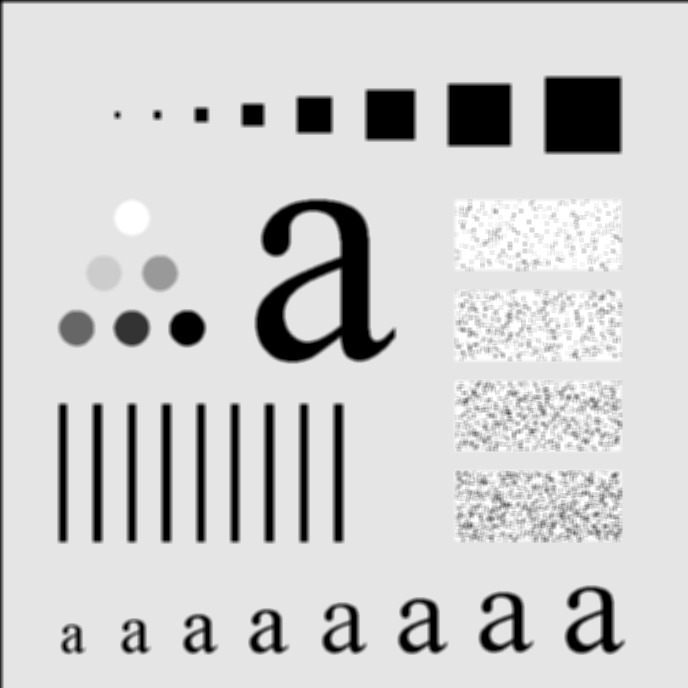
\includegraphics[width=0.3\textwidth]{q1-averagedtest.png}}\qquad
	\subfloat[Ideal low pass filter ($D_0=50$)]{\label{fig:1c}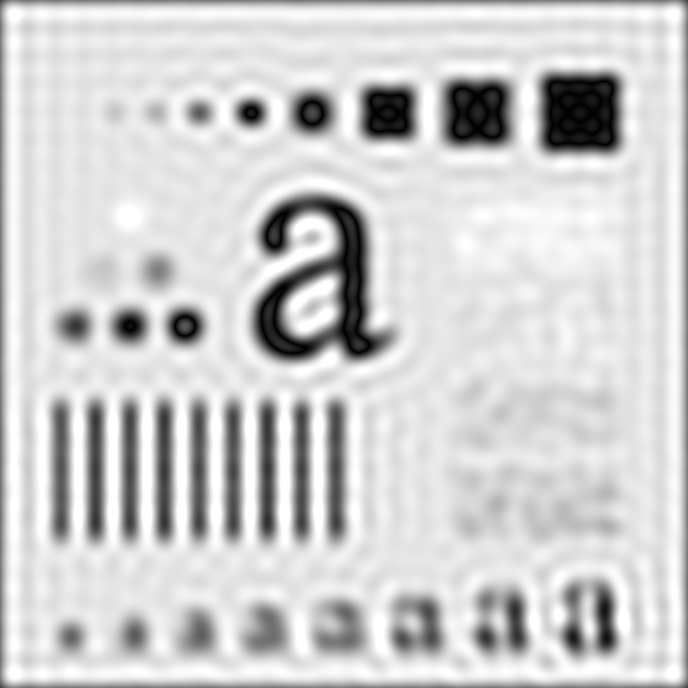
\includegraphics[width=0.3\textwidth]{q1-lptest.png}}
	\caption{Filtering the test image for question 2.1}
	\label{fig:q21}
\end{figure}


\section*{Question 2.2 - Gaussian filters}
For this question I implemented a function `gaussianLowPass' which creates a Gaussian Low Pass filter with the given size P x Q and cutoff frequency $D_0$. I used the definition given in Gonzalez and Woods section 4.8.3. This filter can be also be used to create High Pass filters by subtracting the matrix from 1, and thus also for the High-frequency-emphasis filter.

\subsection*{Low Pass}
Varying the cutoff frequency ($D_0$) with the Gaussian low pass yields the results shown in figure \ref{fig:q221} on the image `barbara.tif'.
\begin{figure}[h]
\centering
	\subfloat[$D_0=50$]{\label{fig:221a}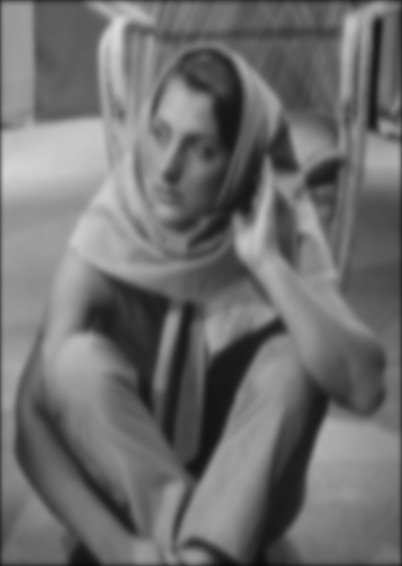
\includegraphics[width=0.2\textwidth]{q2-lowpass-50.png}}\qquad
	\subfloat[$D_0=100$]{\label{fig:221b}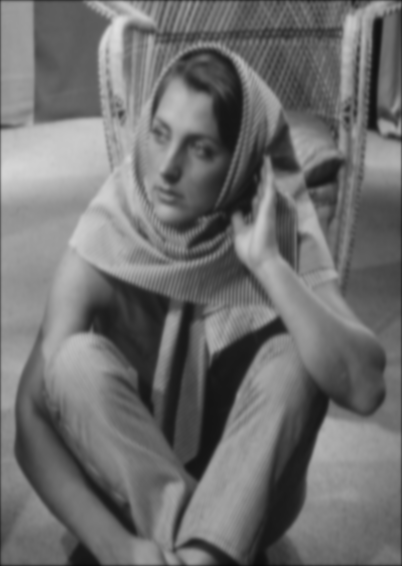
\includegraphics[width=0.2\textwidth]{q2-lowpass-100.png}}\qquad
	\subfloat[$D_0=150$]{\label{fig:221c}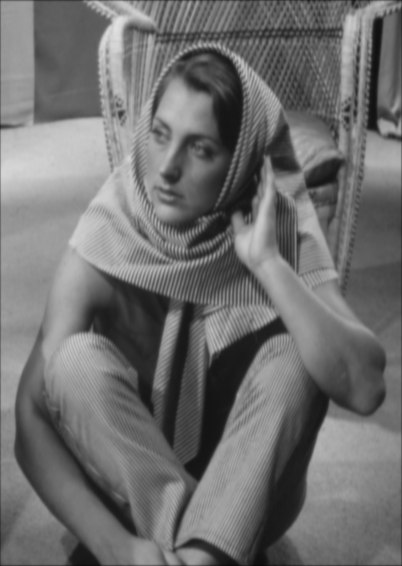
\includegraphics[width=0.2\textwidth]{q2-lowpass-150.png}}\qquad
	\subfloat[$D_0=200$]{\label{fig:221d}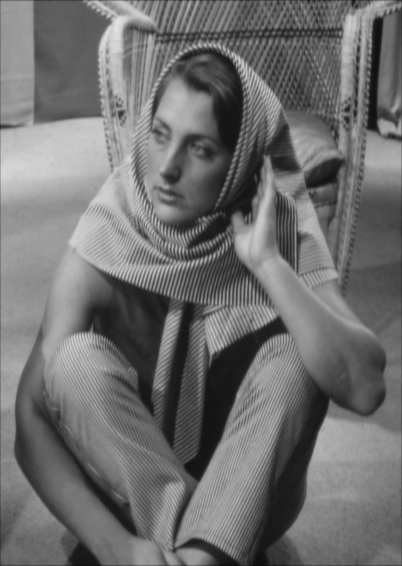
\includegraphics[width=0.2\textwidth]{q2-lowpass-200.png}}\qquad
	\caption{Gaussian Low Pass with varying $D_0$}
	\label{fig:q221}
\end{figure}
Clearly, the apparent sharpness of the filtered image increases as the cutoff frequency increases. The low pass filter essentially removes frequencies above the cutoff value. Therefore if it is set low, nearly all higher frequency details will be ``cut off''. As the cutoff reaches the maximum, more and more details are included in the filtered image.
In figure \ref{fig:221a} the image appears soft, but Barbara is still recognisable. If an object-detection algorithm ran on this image it would not be too impaired by high frequency patterns (for example on the trousers.) The final image in the series includes nearly all the patterns on the trousers and scarf, and this could cause problems for some algorithms.

\subsection*{High Pass}
\begin{figure}[h]
\centering
	\subfloat[$D_0=50$]{\label{fig:222a}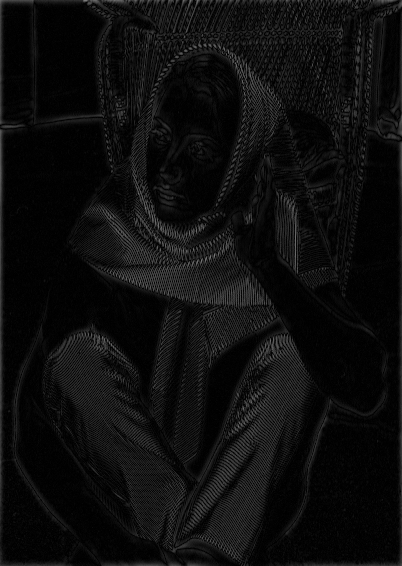
\includegraphics[width=0.2\textwidth]{q2-highpass-50.png}}\qquad
	\subfloat[$D_0=100$]{\label{fig:222b}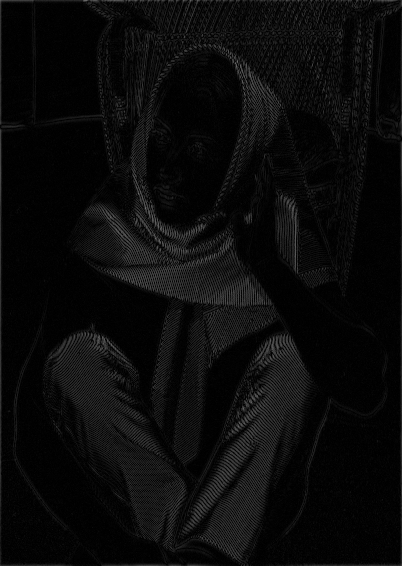
\includegraphics[width=0.2\textwidth]{q2-highpass-100.png}}\qquad
	\subfloat[$D_0=150$]{\label{fig:222c}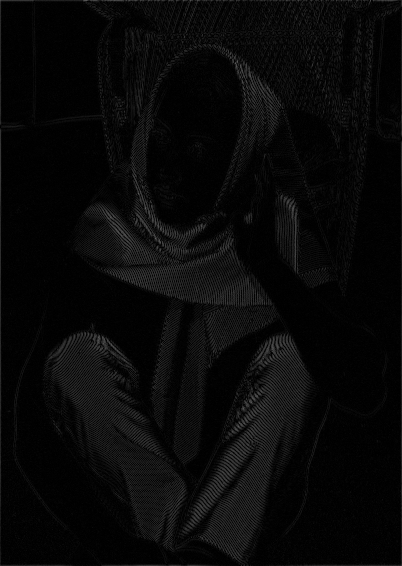
\includegraphics[width=0.2\textwidth]{q2-highpass-150.png}}\qquad
	\subfloat[$D_0=200$]{\label{fig:222d}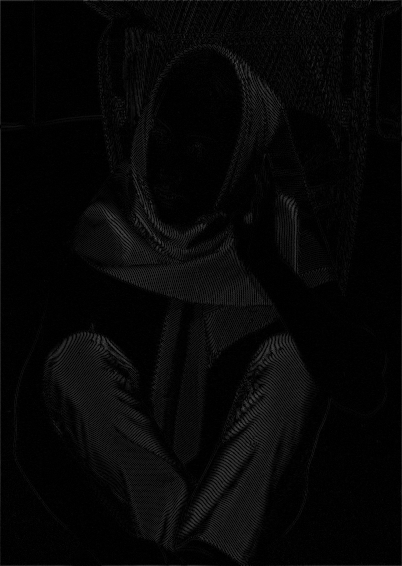
\includegraphics[width=0.2\textwidth]{q2-highpass-200.png}}\qquad
	\caption{Gaussian High Pass with varying $D_0$}
	\label{fig:q222}
\end{figure}

Rather than filtering out high frequencies like the Low Pass filter, the Gaussian High Pass filter removes low frequency detail. The larger the value of the cutoff $D_0$, the more low frequency details are removed. Looking closely at figure \ref{fig:q222}, it can be seen that fewer details are included as $D_0$ increases. The facial details are already removed at $D_0 = 100$ and it is mainly fabric detail which remains in the final image.

\subsection*{High-frequency emphasis}
The high-frequency-emphasis (HFE) filter is a function of the Gaussian High Pass filter: $1 + k * H_{hp} (u,v)$ (section 4.9.5 in Gonzalez and Woods).
The parameter k determines whether the filter acts as an `unsharp mask' or a `high boost' filter.

The name of the filter suggests that this filter will enhance the presence of fine details in an image. Therefore, in theory, if an image has had the high frequency detail removed (for example by a Low Pass filter) then the HFE filter will emphasise the remaining fine details. It cannot `bring back' fine details that have been cut off, but can exaggerate those which remain.

The result of applying the HFE filter ($k=1$) to the image of Barbara in figure \ref{fig:221b}  ($D_0 = 100$) is shown in figure \ref{fig:223b}. The result is a slight sharpening, but the image is not restored to the same level as the original, shown in figure \ref{fig:223c}. In particular, the trousers are lacking texture. On the other hand, some of the background detail has been restored by the filtering, and Barbara's face is noticeably sharper. Increasing the value of $k$ (creating the High Boost filter) does appear to recover more sharpness, as shown in figure \ref{fig:223d}. There are more artefacts and a slight jaggedness, but the image looks better next to the original when this document is downscaled (there appears to be a Moir� pattern on my computer). The facial details actually appear sharper in \ref{fig:223d} than in the original, whereas the higher frequency details which were removed by the low pass (for example the trouser pattern) are pleasingly smoothed.
\begin{figure}[h]
\centering
	\subfloat[Low pass $D_0 = 100$]{\label{fig:223a}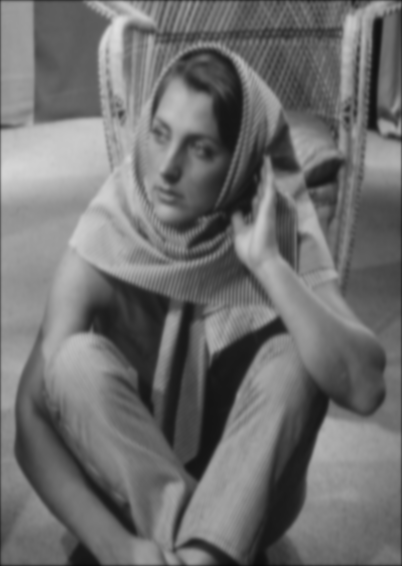
\includegraphics[width=0.2\textwidth]{q2-lowpass-100.png}}\qquad
	\subfloat[`Unsharp mask' HFE applied to the low pass image ($k=1$, $D_0 = 100$)]{\label{fig:223b}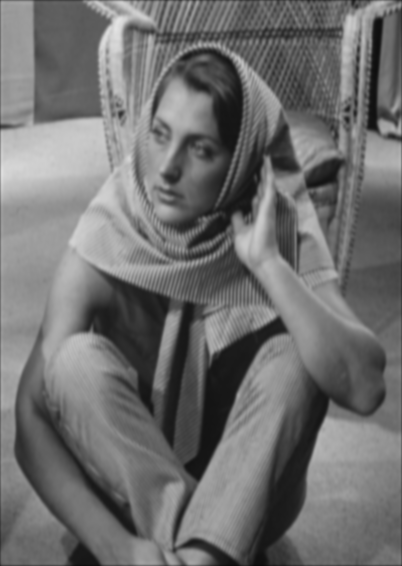
\includegraphics[width=0.2\textwidth]{q2-hfe-100.png}}\qquad
	\subfloat[`High boost' HFE ($k=3$, $D_0 = 100$) ]{\label{fig:223d}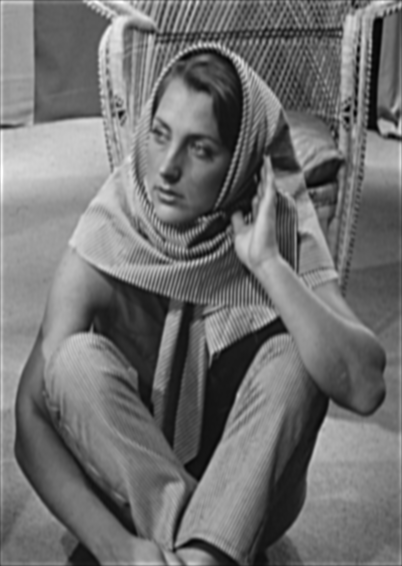
\includegraphics[width=0.2\textwidth]{q2-hfe-k3-100.png}}\qquad
	\subfloat[Original image]{\label{fig:223c}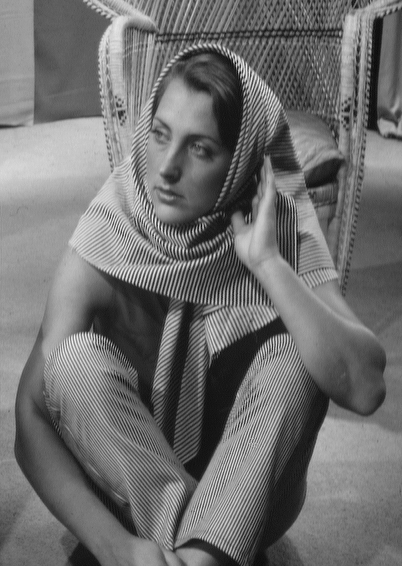
\includegraphics[width=0.2\textwidth]{q2-barbara.png}}
	\caption{Gaussian High Frequency Emphasis applied to a Low Pass filtered image}
	\label{fig:q223}
\end{figure}


\section*{Question 2.3 - Image resampling}
\subsection*{Downsampling}
Taking the naive approach of discarding rows and columns between every 4th row and column, the result shown in figure \ref{fig:231a} was obtained. Note the aliasing patterns which were not present in the original. As the aliasing is caused by sampling at a lower rate than (2 x maximum frequency), it makes sense to try and remove it by reducing the maximum frequency of the original image before resampling. 

I removed the high frequency detail using a Gaussian low pass filter before applying the same reduction. The result is shown in figure \ref{fig:231b} and the similar result after using the 5 x 5 averaging filter is in figure \ref{fig:231c}. These two reductions are noticeably blurry compared to the naive reduction. I then tried applying an unsharp mask to the Gaussian low pass filtered reduction, resulting in figure \ref{fig:231d}. This version has recovered the appearance of sharpness which the former conversions lost. I experimented with values for $D_0$ and fount that above a certain value (~75) no further sharpness could be achieved, but below ~40 the smoother areas of the image gain in contrast and don't resemble the original resolution image.

\begin{figure}[h]
\centering
	\subfloat[Simple reduction]{\label{fig:231a}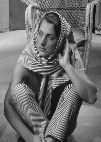
\includegraphics[width=0.2\textwidth]{q3-shrunk-aliased.png}}\qquad
	\subfloat[Gaussian Low Pass before reduction  ($D_0 = 100$)]{\label{fig:231b}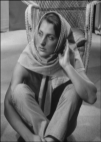
\includegraphics[width=0.2\textwidth]{q3-shrunk-anti-aliased-1.png}}\qquad
	\subfloat[5x5 averaging applied before reduction]{\label{fig:231c}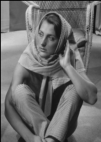
\includegraphics[width=0.2\textwidth]{q3-shrunk-anti-aliased-2.png}}\qquad
	\subfloat[Gaussian LP applied before downsampling, HFE with $D_0 = 50, k =1$ after]{\label{fig:231d}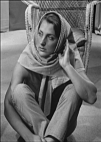
\includegraphics[width=0.2\textwidth]{q3-shrunk-anti-aliased-3.png}}
	\caption{Downsampling with various anti-aliasing methods}
	\label{fig:q231}
\end{figure}

\subsubsection*{Spectrum}
Figure \ref{fig:q232} shows the Fourier transform spectrum of the downsampled image without and with antialiasing. It is clear that the anti-aliased version has de-emphasised the higher frequencies in the image (it gets darker further from the centre).
\begin{figure}[h!]
\centering
	\subfloat[Frequency Spectrum (simple reduction)]{\label{fig:232a}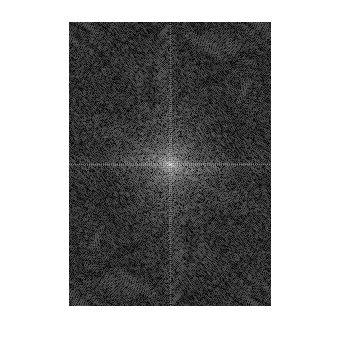
\includegraphics[width=0.4\textwidth]{q3-shrunk-aliased-spectrum.png}}
	\subfloat[Frequency Spectrum (Gaussian Low Pass applied before downsampling)]{\label{fig:232b}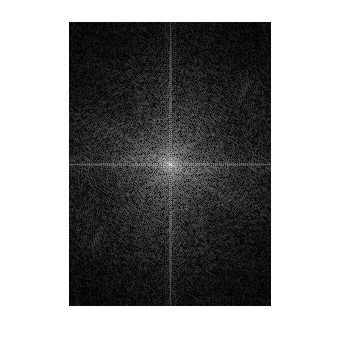
\includegraphics[width=0.4\textwidth]{q3-shrunk-anti-aliased-1-spectrum.png}}\
		\caption{Downsampling - Frequency spectra}
	\label{fig:q232}
\end{figure}

\subsection*{Upsampling}
In the case of upsampling, as described in the question, zeros can be added between the original values to create a padded version. This creates an image which is overall much darker, especially when zoomed in (pixels of value 0 are black)), shown in figure \ref{fig:233a}. The display will vary according to your display (print or screen, scaling etc. all have an effect). Run the cell titled ``Upsampling'' in the file q3.m in order to see the three images in full size.

The frequency spectrum after up sampling contains 9 copies of the original spectrum; in other words the frequency has been mirrored by 3 in both the X and Y direction.

As described in the lecture slides, a low pass filter may be used to remove the mirroring. In figure \ref{fig:q234} I have applied the Gaussian Low Pass filter to the image from \ref{fig:233a}. This has the effect of blurring away the black areas and therefore interpolation. The corresponding frequency spectrum shows the original frequency spectrum (mirroring removed) and it is clear that little or no extra high frequency detail has been added (outside the central area the spectrum is almost entirely empty).

\begin{figure}[h!]
\centering
	\subfloat[Simple upsampling]{\label{fig:233a}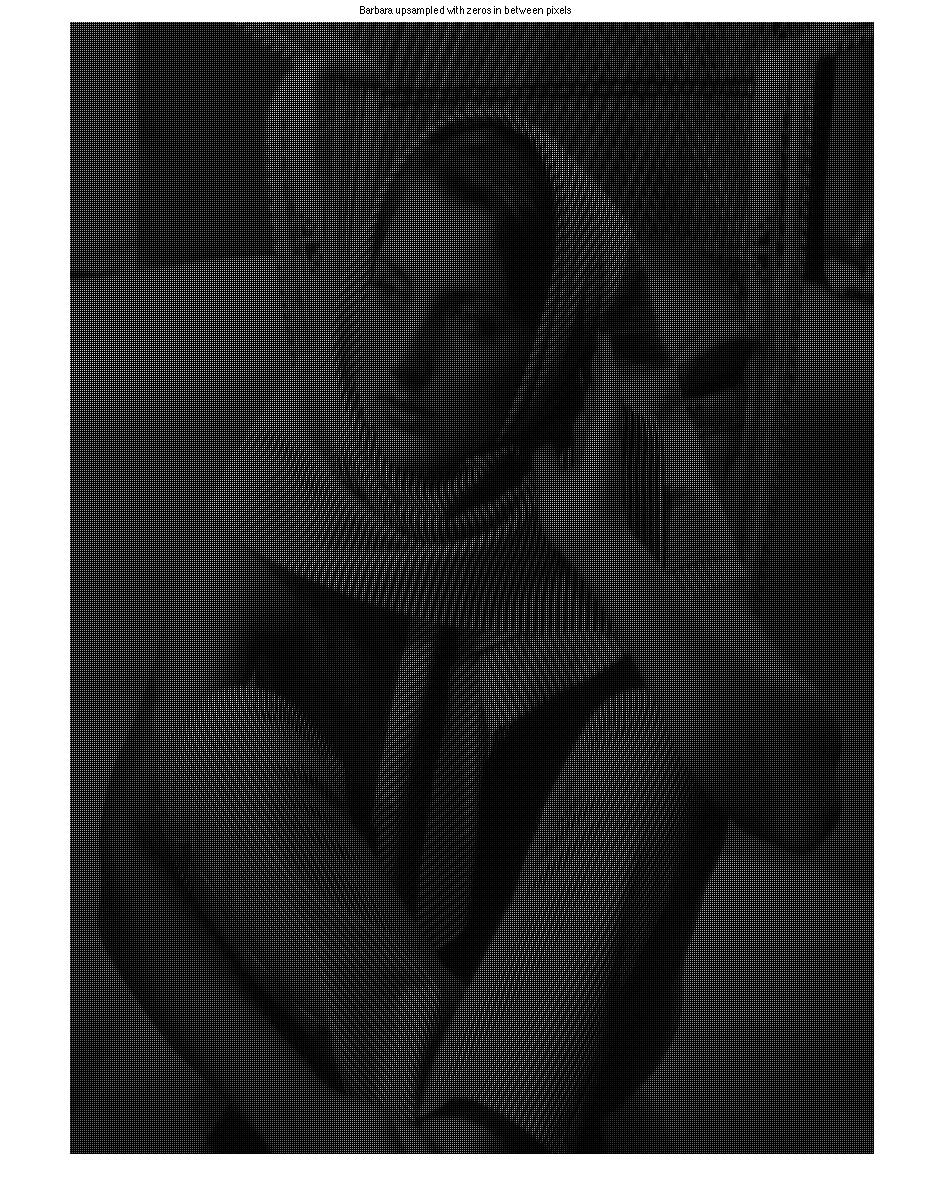
\includegraphics[width=0.25\textwidth]{q3-enlarged-basic.png}}\qquad
	\subfloat[Frequency Spectrum, original]{\label{fig:233b}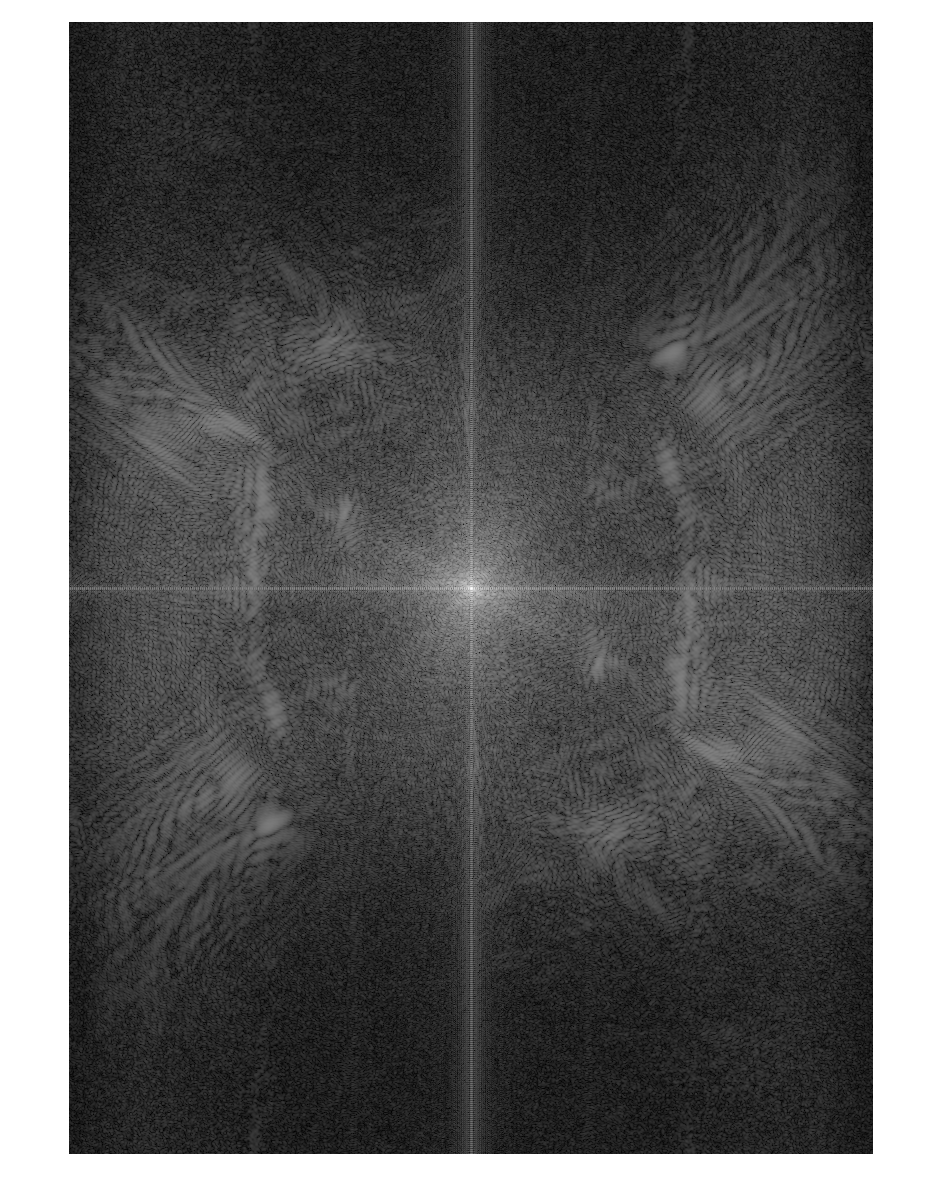
\includegraphics[width=0.25\textwidth]{q3-enlarged-spectrumorig.png}}
	\subfloat[Frequency Spectrum, upsampled]{\label{fig:233c}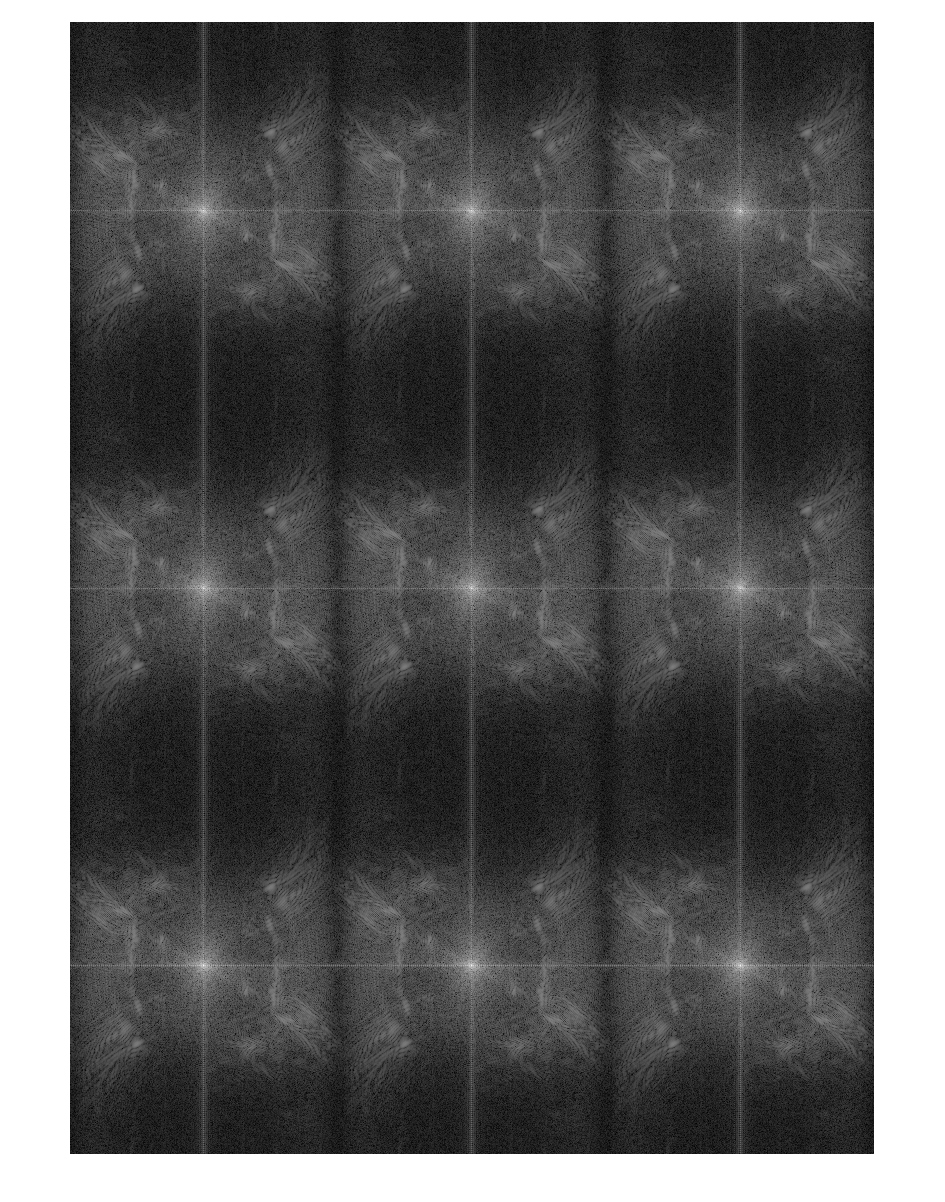
\includegraphics[width=0.25\textwidth]{q3-enlarged-spectrum-up.png}}
		\caption{Upsampling and frequency spectra}
	\label{fig:q233}
\end{figure}

\begin{figure}[h!]
\centering
	\subfloat[Upsampling with a Gaussian Low Pass ($D_0 = 200$)]{\label{fig:234a}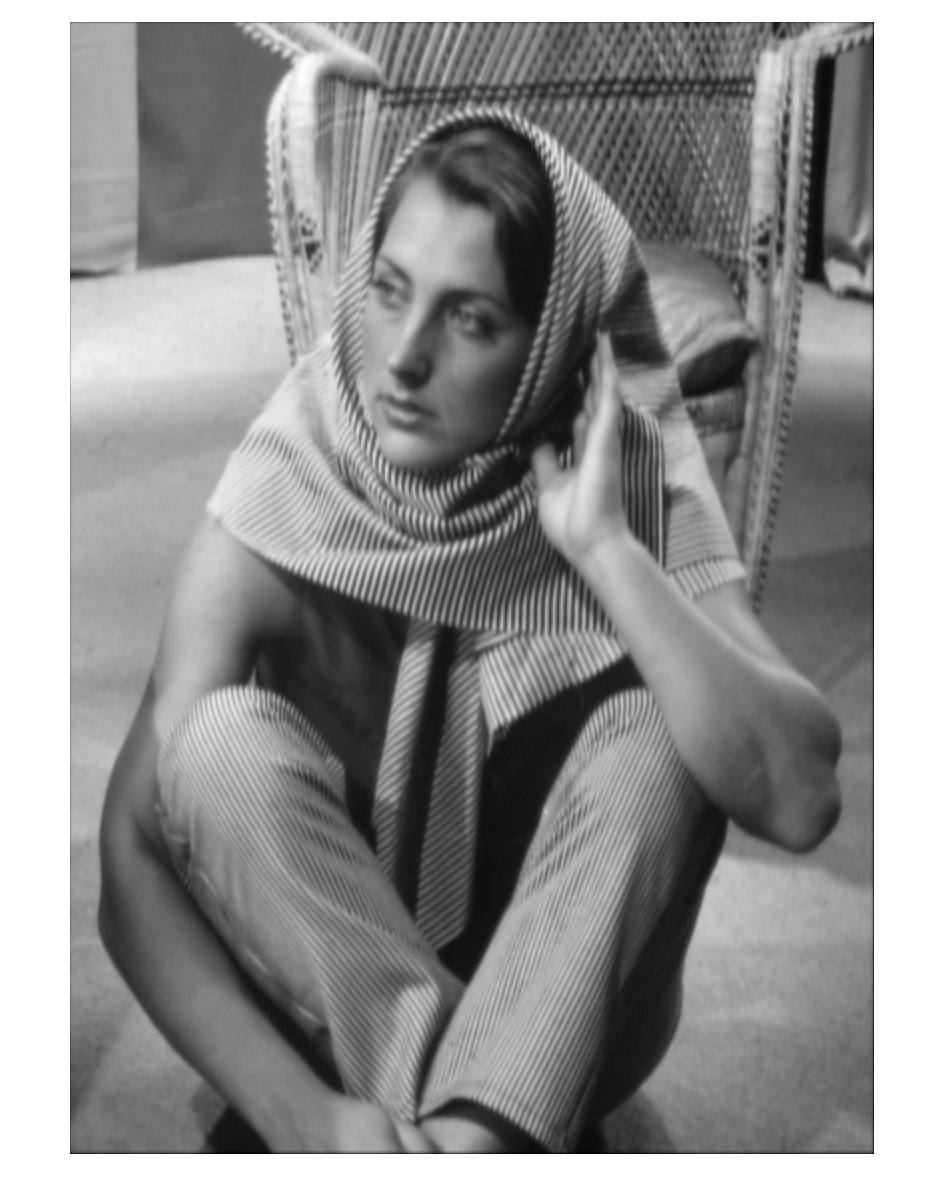
\includegraphics[width=0.4\textwidth]{q3-enlarged-lp.png}}\qquad
	\subfloat[Corresponding frequency spectrum]{\label{fig:234b}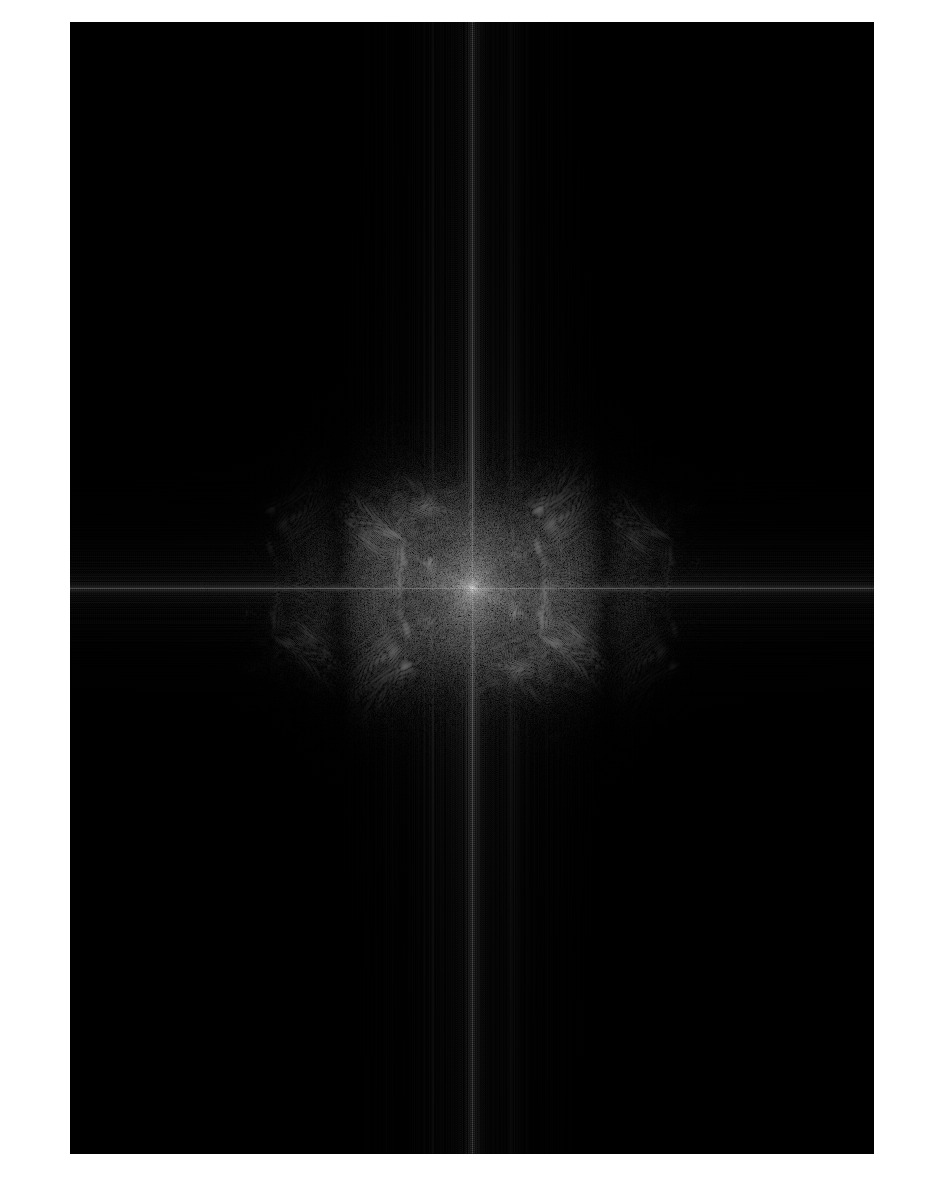
\includegraphics[width=0.4\textwidth]{q3-enlarged-lp-spectrum.png}}\qquad
		\caption{Upsampling followed by GLPF}
	\label{fig:q234}
\end{figure}

I found through experimenting with the cutoff that a value of ~200 was optimal. Above 210, and stripes remained visible. Below 200, the image became increasingly blurry (i.e. the frequencies of the upscaled image were removed).


\section*{Question 2.4}

\subsection*{Interference patterns}
The image `interference.tif' has several patterns of interference on top of the image of a woman with very large ornate earrings.
The first pattern I notice is a banding or stripes which move on the diagonal - they appear to be a low frequency waveform. As well as this there is a fine pattern of a repeating texture all over the image which comprises some vertical stripes.

The first step I would take in determining the interference is to product a spectrum of the frequency domain. This is shown in figure \ref{fig:241b}. There is a lot of noise all over the spectrum, but there are clearly peaks at the left and right near the vertical centre, and a repeating dashed-pattern along the central axes. There is additionally a thin line on either side of each central axis.

\subsection*{Removal of the repeating patterns}
According to Gonzalez and Woods section 4.10, selective filtering can be achieved using notch filters and Band pass/reject filters.  A notch filter is a product of high pass filters which have been translated to the centre of a notch (a point in the frequency domain). The problem is first to identify the centres from the frequency spectrum, then to create a filter from those centres and apply it to the image.

I spent a long time trying to find the coordinates of the centres, and eventually managed to use ginput as the question suggested. When running the script q4.m, the frequency spectrum will pop up and wait. Then the user must click on the peaks of the high frequencies outside the centre, finally pressing Enter to continue the script.

The result and spectrum of my first successful attempt is shown in figure \ref{fig:242a}. There still remains a little of the low frequency pattern at the edges, and the overall image is noisy. I repeated and tried to be more precise with my clicking.
\begin{figure}[h]
\subfloat[Interfered image]{\label{fig:241a}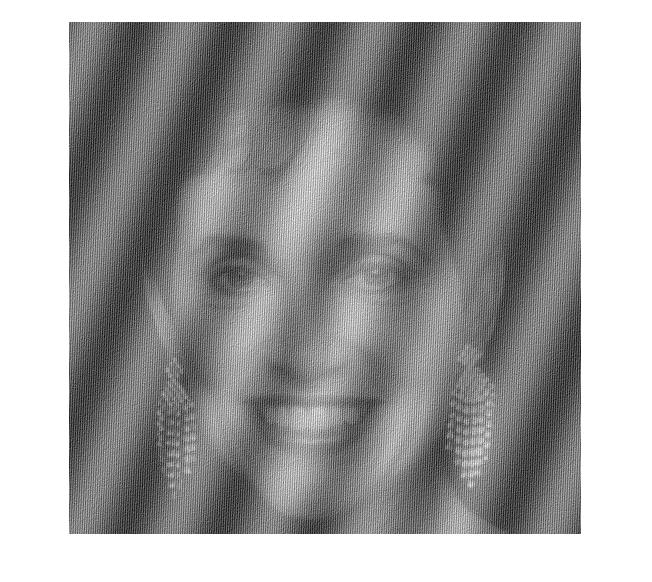
\includegraphics[width=0.5\textwidth]{q4-interference.png}}\qquad
	\subfloat[Corresponding frequency spectrum]{\label{fig:241b}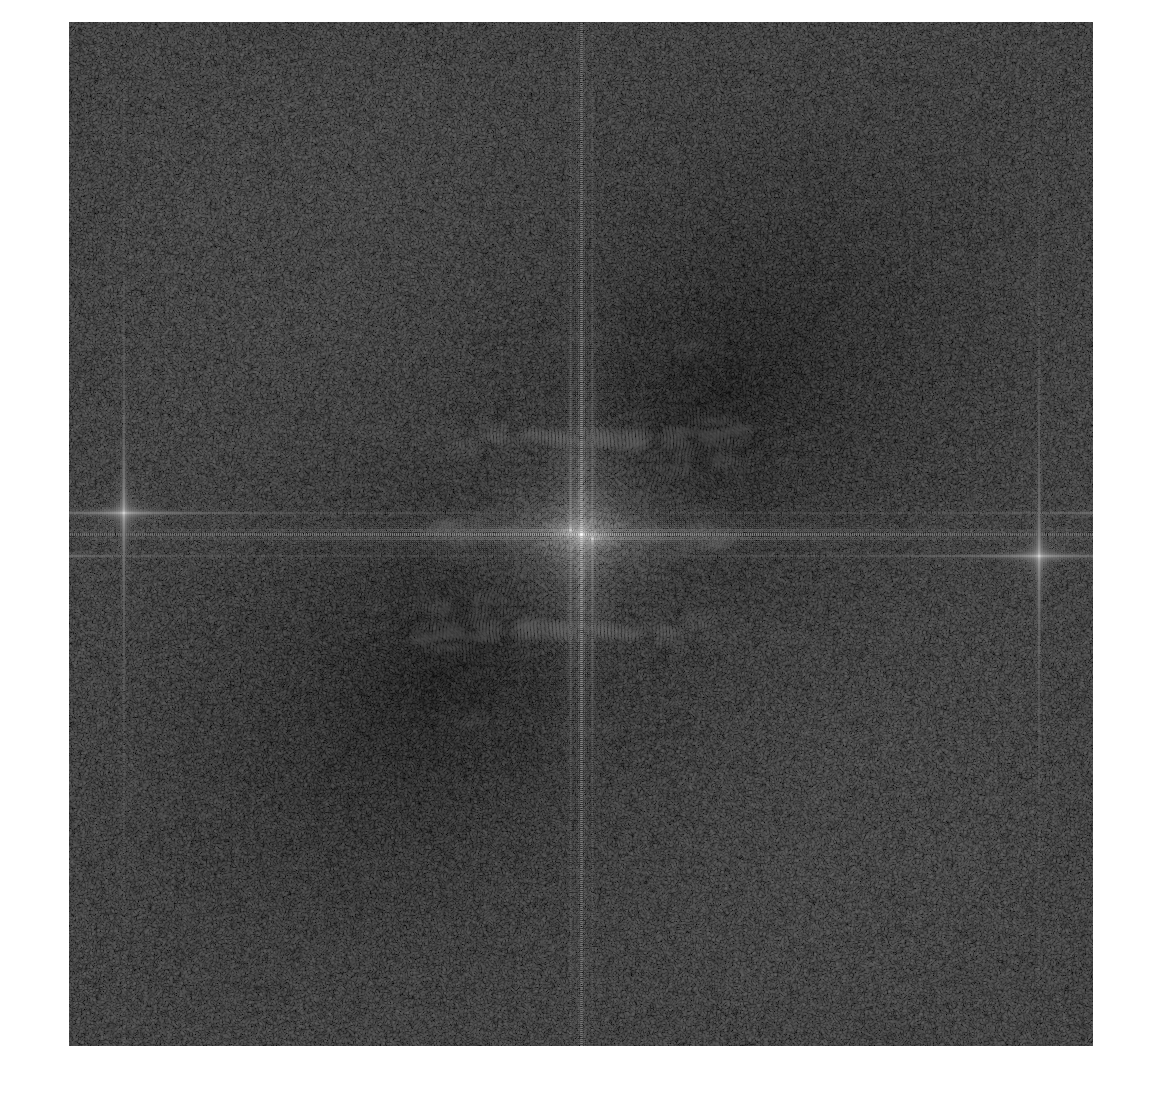
\includegraphics[width=0.5\textwidth]{q4-interference-spectrum.png}}\qquad


	\subfloat[Filtered image]{\label{fig:242a}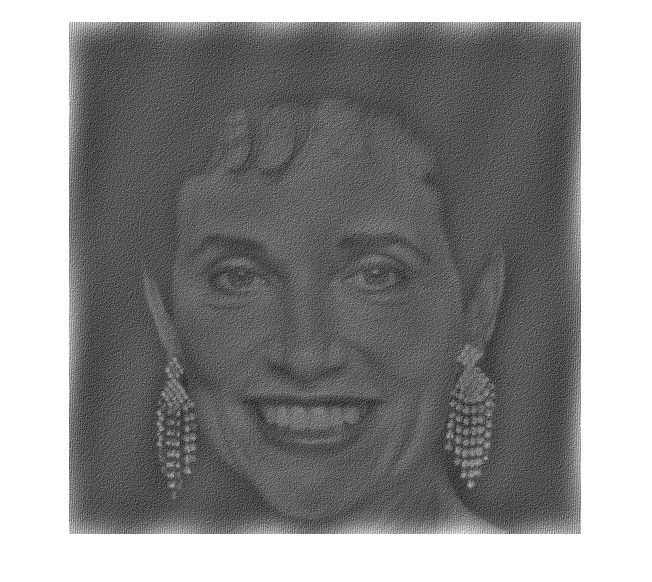
\includegraphics[width=0.5\textwidth]{q4-filtered-d0-10.png}}\qquad
	\subfloat[Corresponding frequency spectrum]{\label{fig:242b}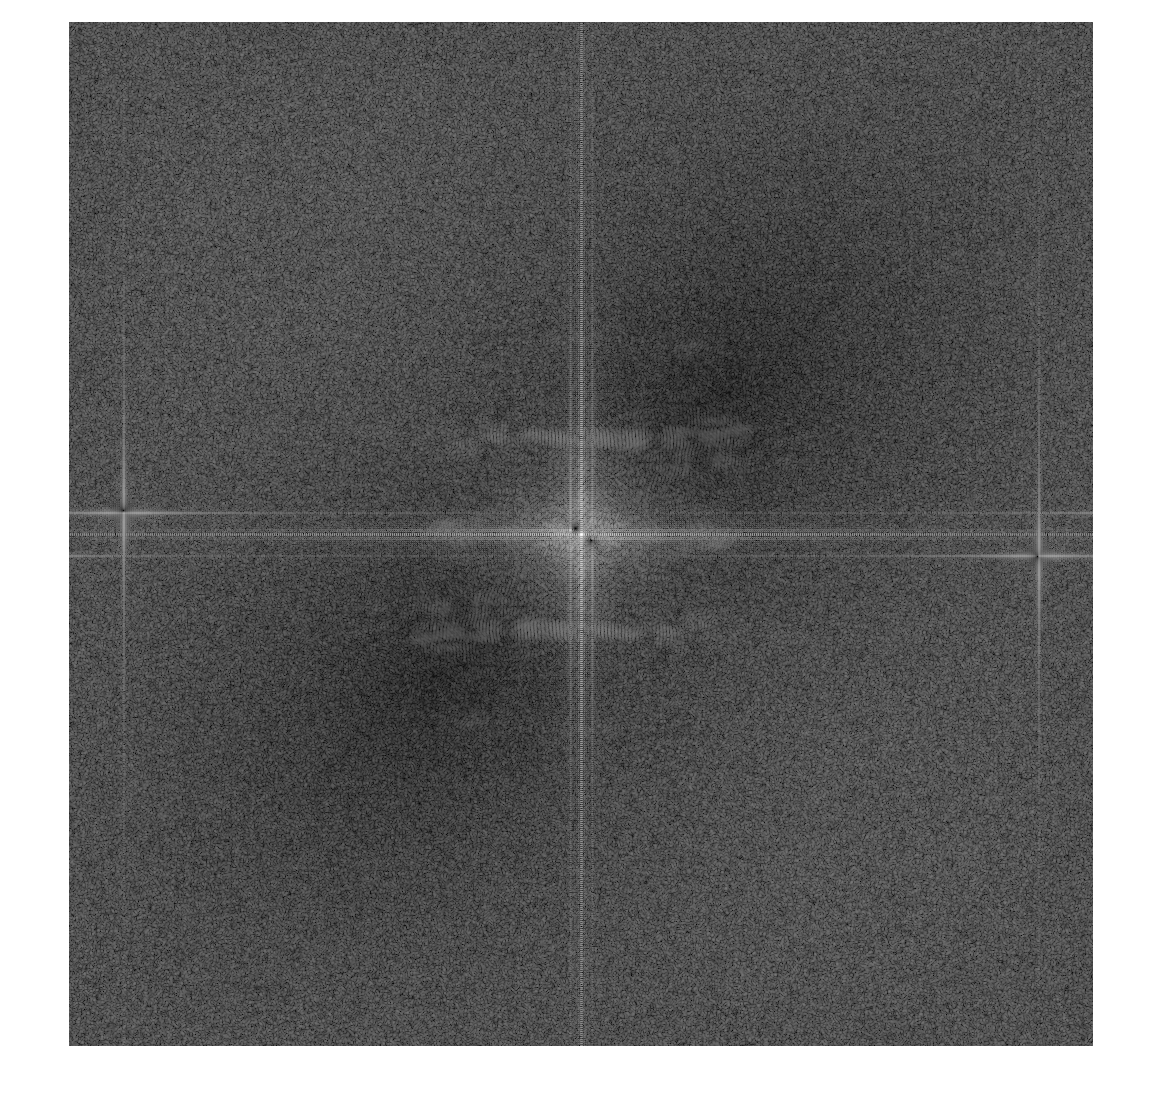
\includegraphics[width=0.5\textwidth]{q4-filtered-d0-10-spectrum.png}}\qquad
	
	\subfloat[Filtered image (attempt 2)]{\label{fig:242c}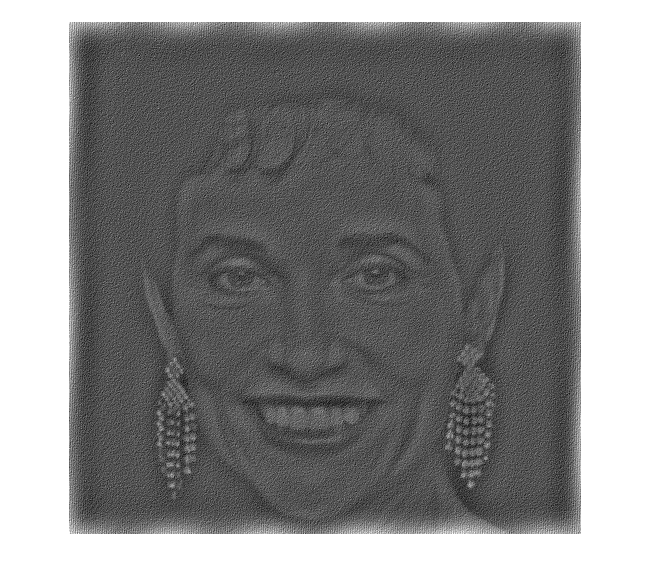
\includegraphics[width=0.5\textwidth]{q4-filtered-d0-10-2.png}}\qquad
	\subfloat[Corresponding frequency spectrum]{\label{fig:242d}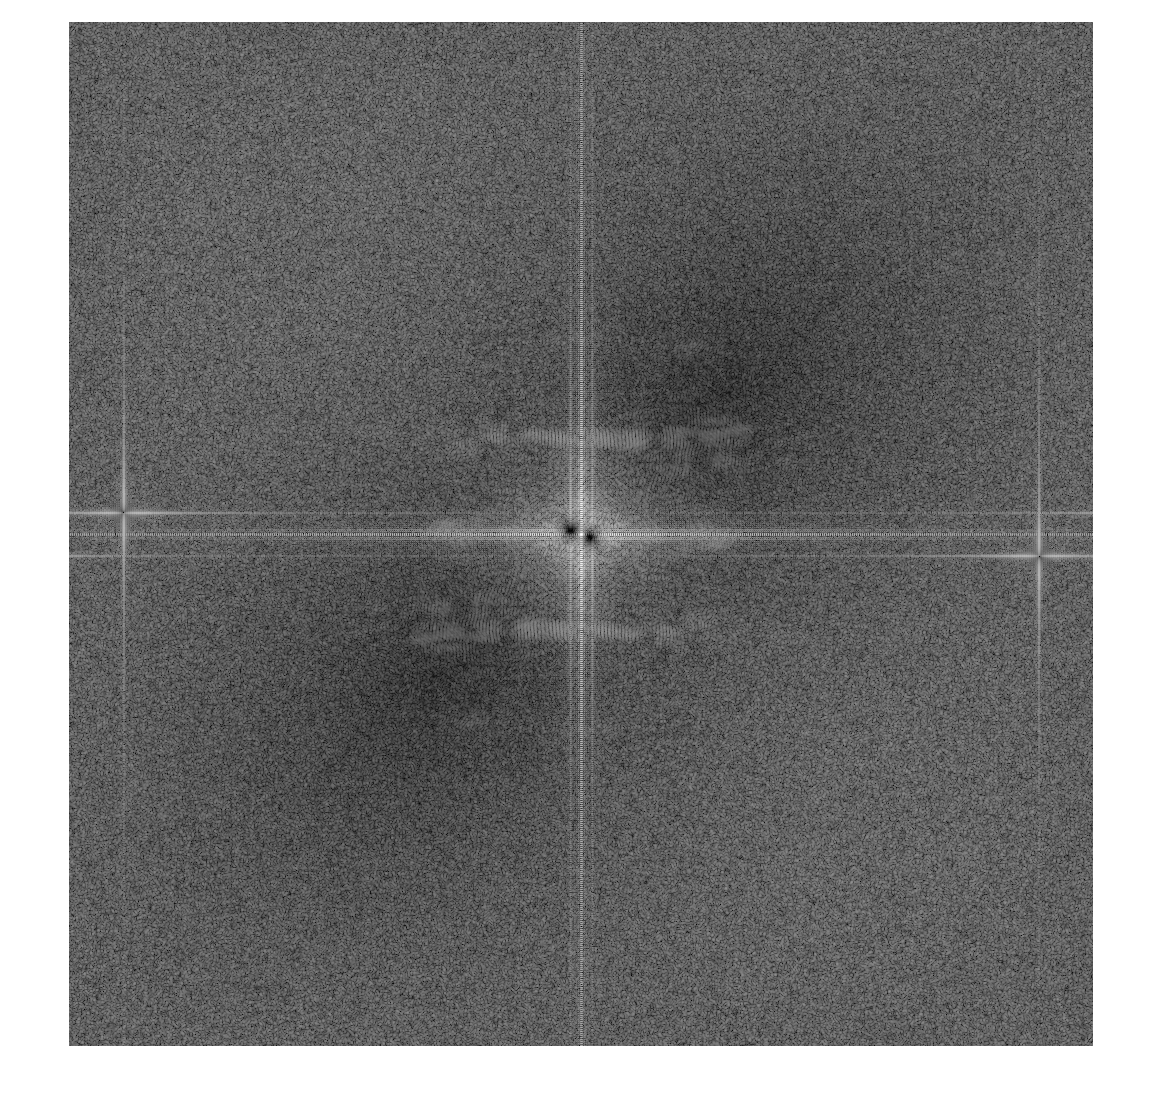
\includegraphics[width=0.5\textwidth]{q4-filtered-d0-10-2-spectrum.png}}\qquad

	\caption{Notch filtered image}
	\label{fig:success}
\end{figure}

After the notch filter has been applied, there remains plenty of noise in the image. As noise is essentially high-frequency detail, I experimented with a Gaussian low pass filter to remove it from the image shown on figure \ref{fig:242c}. The result is shown in figure \ref{fig:success2}, with a lighter version to aid seeing the details. As can easily be seen, the image is now a lot darker and lacking in edge contrast, making it hard to detect the edge of the woman's face. Some of the ridiculous earring detail has also been lost in this attempt at noise removal.


\begin{figure}[h]
	\subfloat[Low pass filtered image]{\label{fig:243a}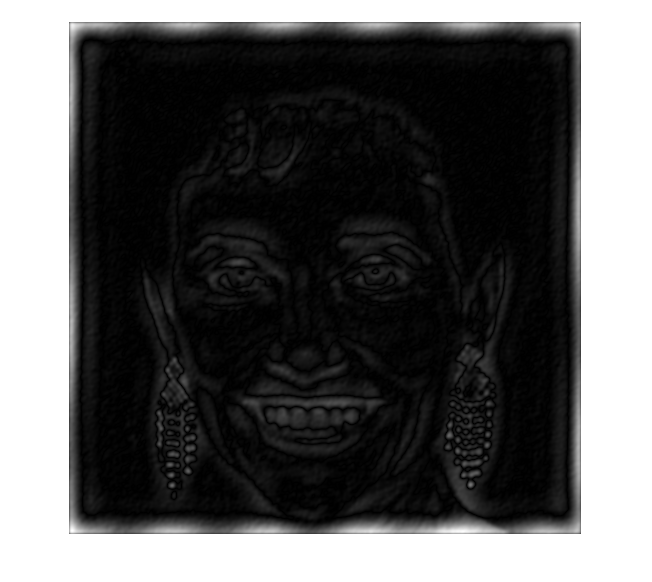
\includegraphics[width=0.5\textwidth]{q4-filtered-d0-10-2-lp100.png}}
	\subfloat[Lightened version ]{\label{fig:243b}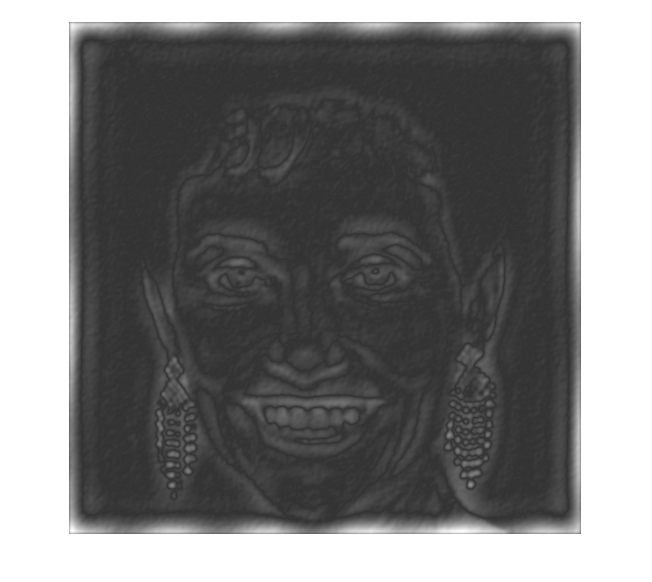
\includegraphics[width=0.5\textwidth]{q4-filtered-d0-10-2-lp10-lighter.png}}
	\caption{Notch filtered image}
	\label{fig:success2}
\end{figure}

\end{document}